\documentclass[preprint2,numberedappendix,tighten,twocolappendix]{aastex6}  % USE THIS TO MAKE BIB, THEN FORMAT USING EMULATEAPJ
%\documentclass[twocolumn,apj,numberedappendix]{emulateapj}
\shorttitle{Epoch of Reionization Power Spectrum Results from PAPER-128}
\shortauthors{Cheng}

\usepackage{amsmath}
\usepackage{graphicx}
\usepackage[figuresright]{rotating}
\usepackage{natbib}
\usepackage{ctable}
\citestyle{aa}

%		Math Shortcuts from Adrian
%\def\b{\mathbf{b}}
%\def\k{\mathbf{k}}
%\def\r{\mathbf{r}}
%\def\q{\mathbf{q}}
%\def\b{\mathbf{b}}
%\def\kp{\mathbf{k}^\prime}
%\def\kpp{\mathbf{k}^{\prime\prime}}
%\def\V{\mathbb{V}}
%\def\At{\tilde{A}}
%\def\Vt{\tilde{V}}
%\def\Tt{\tilde{T}}
%\def\tb{\langle T_b\rangle}
%\newcommand{\vis}{\mathbf{v}}
%\newcommand{\x}{\mathbf{x}}
%\newcommand{\xhat}{\hat{\mathbf{x}}}
%\newcommand{\nhat}{\hat{\mathbf{n}}}
%\newcommand{\A}{\mathbf{A}}
%\newcommand{\N}{\mathbf{N}}
%\newcommand{\rhat}{\hat{\mathbf{r}}}
%\newcommand{\khat}{\hat{\mathbf{k}}}
%\newcommand{\btheta}{\boldsymbol \theta}

\newcommand{\cc}[1]{{\color{purple} \textbf{[#1]}}}

\begin{document}
\title{Epoch of Reionization Power Spectrum Results from PAPER-128}

\author{
%Aaron R. Parsons\altaffilmark{1,2},
%Adrian Liu\altaffilmark{1,2},
%James E. Aguirre\altaffilmark{3},
%Zaki S. Ali\altaffilmark{1},
Carina Cheng\altaffilmark{1}
%Daniel C. Jacobs\altaffilmark{8},
%David F. Moore\altaffilmark{3},
%Jonathan C. Pober\altaffilmark{1},
}


%		Notes	
	
%Reference section with: \ref{sec:Intro}
%Reference equation with: \eqref{eq:eqtest}
%Reference figure with: \ref{fig:figtest}
%Cite paper inside sentence: \citet{ref}
%Cite paper at end of sentence: \citep{ref}
%Cite paper inside a parenthetical sentence: \citealt{ref}

%To compile with references shown, compile in BibTeX once and LaTeX twice


%		Sample Equation Syntax
%\begin{equation}
%\label{eqtest}
%\langle \widetilde{T} (\mathbf{k}) \widetilde{T}^* (\mathbf{k^\prime}) \rangle = (2 \pi)^3 \delta^D (\mathbf{k} - \mathbf{k}^\prime) P(k),
%\end{equation}


\altaffiltext{1}{Astronomy Dept., U. California, Berkeley, CA}
%\altaffiltext{2}{Hubble Fellow}
%\altaffiltext{2}{Radio Astronomy Lab., U. California, Berkeley, CA}
%\altaffiltext{3}{Berkeley Center for Cosmological Physics, Berkeley, CA}
%\altaffiltext{3}{Dept. of Physics and Astronomy, U. Pennsylvania, Philadelphia, PA}
%\altaffiltext{8}{School of Earth and Space Exploration, Arizona State U., Tempe, AZ}

\begin{abstract}
\cc{I can write comments like this!}
\end{abstract}


\section{Introduction}
\label{sec:Intro}

\cc{Need to cite papers...}

The Epoch of Reionization (EoR) represents an uncharted phase in cosmic history when the first stars and galaxies ionized the neutral hydrogen present in the early Universe. During this time, it is believed that baryonic matter fell into dark matter potential wells, gravitationally collapsing into the first luminous structures. These sources, possibly quasars or young dwarf galaxies, emit radiation that ionized the abundant hydrogen in the intergalactic medium (IGM). The subsequent formation of a web of galaxies across an ionized IGM is thought to represent the large scale structure that we observe today.

The EoR has not yet been directly detected. However, constraints have been made on its timing and duration through different methods. As reionization progressed, the number of free electrons susceptible to Thompson scattering increased, resulting in scattered cosmic microwave background (CMB) photons whose imprint has been left on CMB observations. In particular, the Thompson scattering optical depth parameter $\tau$ is a useful metric for characterizing the duration of reionization. Recent Planck measurements of $\tau$ suggest a late reionization history, occurring between redshifts of $7.7$ and $8.7$.

Galaxy observations have also begun to place constraints on the EoR. With their high luminosities, quasars make for powerful probes of the state of the IGM through absorption line studies. As photons from a quasar are redshifted, they may be absorbed by neutral hydrogen at the Lyman-$\alpha$ line, producing Gunn-Peterson trough features in quasar spectra. Observations of these spectra in high redshift galaxies have signaled the end of reionization by $z ~ 6$, and experiments are continuously pushing galaxy observations to higher redshifts. 

A third powerful probe of the EoR makes use of the $21 cm$ wavelength emission produced by hydrogen due to its two quantum states. Because hydrogen is so pervasive in the Universe and a transition from its spin up state to spin down state gives off a  well-defined energy difference in the form of a $21 cm$ wavelength photon, observations targeting this signal have the potential to trace the EoR from start to finish. However, $21 cm$ experiments face major challenges, including those from bright foregrounds and instrumental systematics. Nevertheless, the observations and analyses of data from current radio telescope arrays have already begun to constrain the $21 cm$ signal and make statements about the nature of the IGM during the EoR. 

Major existing $21 cm$ experiments include both those targeting to measure the sky-averaged `global' $21 cm$ signal and those employing interferometric elements and the use of cross-correlations and statistical power-spectral measurements. Examples of the former are EDGES, the LWA, LEDA, DARE, BigHorns, and SARAS. Major interferometers include the GMRT, LOFAR, the MWA, the 21CMA, and PAPER.

In this paper we present results from the $128$ antenna configuration of the Donald C. Baker Precision Array for Probing the Epoch of Reionization (PAPER). PAPER is a highly redundant array consisting of dual-polarization dipole antennas. Its configuration is optimal for boosting power spectrum sensitivity and the analysis used relies on a foreground avoidance approach where we measure power spectrum values in a region of delay space that is uncontaminated by foregrounds. Previous upper limits on the EoR power spectrum include those made by PAPER-32, which used its redundant configuration to its advantage to obtain an upper limit of $\Delta^{2}(k) \leq (41 mk)^{2}$ at $k=0.28h Mpc^{-2}$. Doubling in array size and employing an updated analysis pipeline that included fringe-rate filtering and an optimal quadratic estimator framework for the power spectrum analysis achieved an upper limit on $\Delta^{2}(k)$ of $(22.4mK)^{2}$ in the range $0.15 < k < 0.5h Mpc^{-1}$ at $z = 8.4$. The result from PAPER-64 was the best published upper limit thus far, with PAPER-128 achieving a factor of ?? in improvement.

PAPER-128 has been able to use much of the same technical analysis framework from previous PAPER analyses, while improving on the limits set by PAPER-64 with a longer observing time, double the number of antennas, and the development of new data quality tests, signal loss simulations, and inverse covariance weighting techniques. 

The organization of the paper is as follows. ...


\section{Observations}
\label{sec:Obs}

\begin{figure}[!]
	\centering
	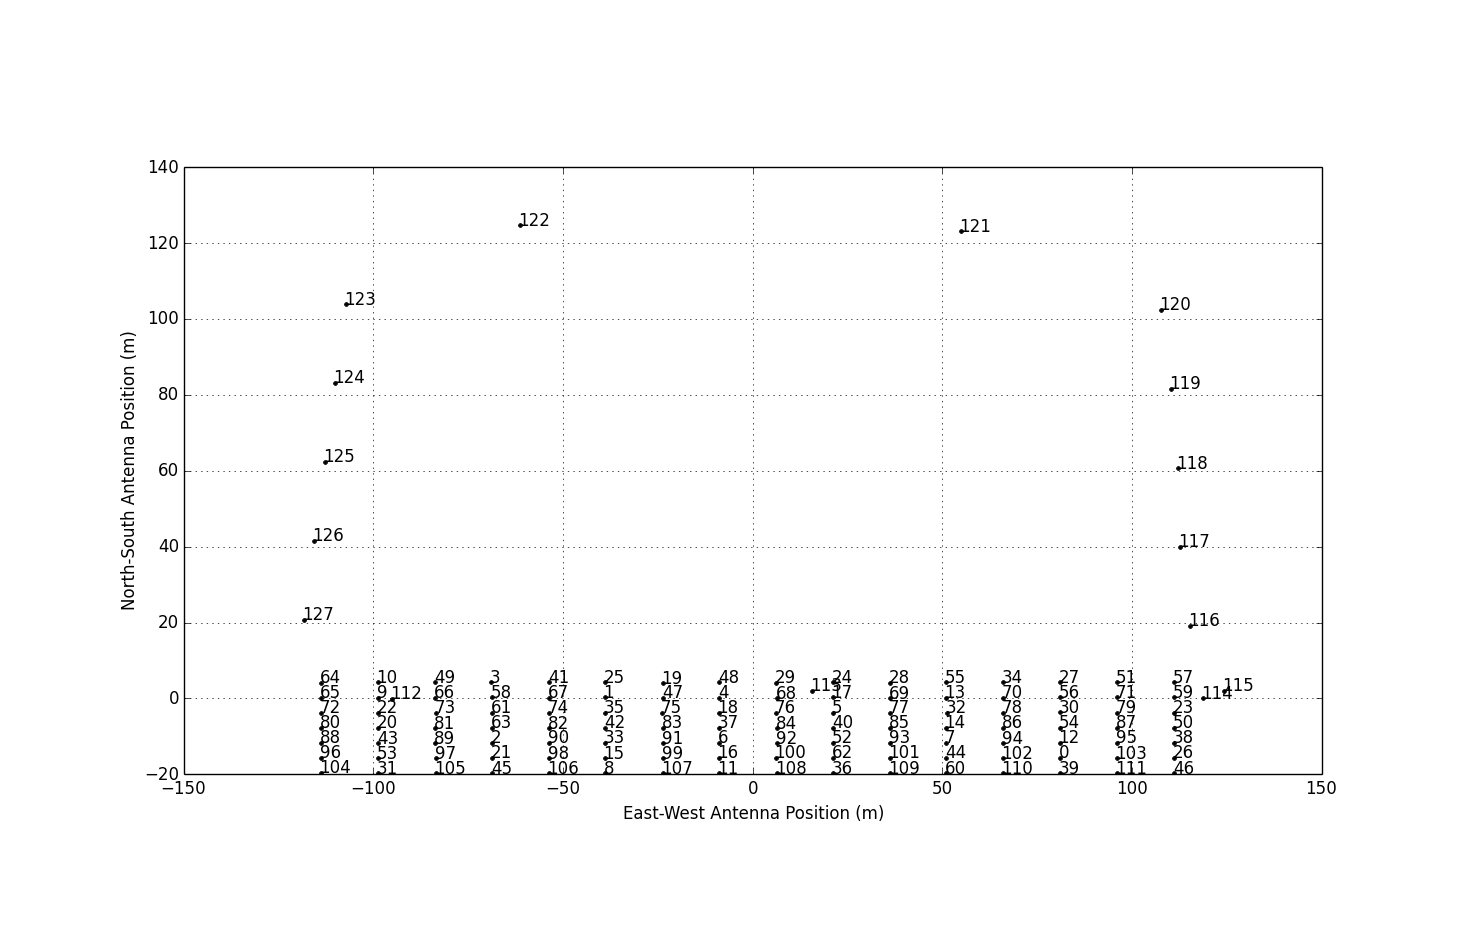
\includegraphics[width=0.52\textwidth]{antlayout.png}
	\caption{\cc{caption here}}
	\label{fig:figtest}
\end{figure}


\section{Data Reduction}
\label{sec:Cal}

\section{Power Spectrum Analysis}
\label{sec:PS}

\subsection{Optimal Quadratic Estimators}
\label{sec:OQE}

\subsection{Signal Loss}
\label{sec:Sigloss}

\section{Results}
\label{sec:Res}

\section{Conclusions}
\label{sec:Con}

\section{Acknowledgements}
\label{sec:Ack}

\bibliographystyle{apj}
\bibliography{refs}


\end{document}

